\FloatBarrier
\section{Precision, predictability and energy}\label{sec:precision}\label{sec:energy}

\subsection{The precision question is a predictability question}
Reduced precision is usually argued from tolerated numerical error. In a chaotic system that
argument is incomplete, because the error a model makes is amplified by the flow itself. If the
local error-doubling time is $\tau$ and the forecast lead is $T$, an initial representation error
$\epsilon_0$ becomes
\begin{equation}
\epsilon(T) \approx \epsilon_0\,2^{T/\tau}.
\end{equation}
A representation with $p$ mantissa bits has $\epsilon_0 \sim 2^{-p}$ relative to the state.
Requiring $\epsilon(T) < \delta$ gives the minimum precision
\begin{equation}
p > \log_2\!\left(\frac{2^{T/\tau}}{\delta}\right) = \frac{T}{\tau} + \log_2\frac{1}{\delta}.
\label{eq:pmin}
\end{equation}
For a 10-day lead, a doubling time of 2.5 days and a 10\% tolerance, $p > 4 + 3.3 = 7.3$ bits.
fp16 has 11 bits and is comfortable; bf16 has 8 and is marginal; fp8 with a 4-bit mantissa is
not viable for the state. This is the analytical prediction, and Section~\ref{sec:validation}
confirms it experimentally: fp16 and bf16 track fp64 to within a few percent of RMSE, fp8
degrades the analysis by an order of magnitude.

The useful consequence is that precision can be spent where it is not needed. In a region where
the ensemble spread is large, the forecast error is already dominated by chaotic uncertainty, and
the marginal value of an extra mantissa bit is zero. The governor uses exactly this test:
\begin{equation}
\text{precision}(i) =
\begin{cases}
\text{fp16}, & \sigma_i > \sigma_{\mathrm{hi}},\\
\text{fp32}, & \sigma_i < \sigma_{\mathrm{lo}},\\
\text{hold}, & \text{otherwise},
\end{cases}
\end{equation}
with hysteresis between $\sigma_{\mathrm{lo}}=0.15$ and $\sigma_{\mathrm{hi}}=0.30$ to prevent
mode thrash. A repair state re-runs flagged cells in fp32 when a block's fp16 fraction exceeds
55\%.

\subsection{Hardware support}
The governor is a per-tile table of 910 precision classes, updated once per kernel by the chaos
monitor. It drives the lane mode registers, which select fp32 (one FMA per lane-cycle), fp16 or
bf16 (two) and fp8 (four) without a pipeline flush. A mode change costs 14 cycles per tile; with
three changes per step that is 0.07\% of the step. The datapath keeps the accumulator in fp32 for
all modes and uses a two-term Kahan compensation for the reduction tree, so that a 256-lane sum
of fp16 products loses no more than 1.2 bits relative to fp32.

The energy model prices the modes at 0.420, 0.240 and 0.140 pJ per operation for fp32, fp16 and
fp8, and the Kahan accumulation at 1.15$\times$ the naive adder energy. The numbers are derived
from published 3 nm arithmetic energies and are varied by $\pm$25\% in the sensitivity study.

\subsection{Evidence from a cycled ensemble}
The experiment is a Lorenz--96 system ($N=40$, $F=8$) with a 32-member ensemble, 20 observations
every 0.04 time units and a stochastic EnKF with 10\% covariance inflation. After a 200-cycle
spin-up the analysis error is \ACAnalRMSE, and six independent 12-day forecasts are verified
against the truth trajectory. Table~\ref{tab:precision} and Fig.~\ref{fig:precision} report the
result.

\begin{table}[t]
\centering\small
\caption{Precision study. Analysis RMSE is the cycled analysis error; day-5 and day-10 RMSE are
forecast errors against the truth. Energy weight is relative to an all-fp32 run for the same work.}
\label{tab:precision}
\begin{tabular}{@{}lrrrr@{}}
\toprule
Mode & Analysis RMSE & Day-5 RMSE & Day-10 RMSE & Energy weight\\
\midrule
fp64 (reference) & \ACAnalRMSE & \ACRMSEdayFive & 2.75 & 2.10\\
fp32 & 0.221 & 1.330 & 2.75 & 1.00\\
fp16 & 0.223 & \ACRMSEfpSixteen & 2.75 & 0.57\\
bf16 & 0.259 & 1.444 & 2.75 & 0.62\\
fp8 e4m3 & 2.767 & 4.141 & 4.10 & 0.33\\
adaptive governor & 0.221 & 1.330 & 2.75 & 0.64\\
\bottomrule
\end{tabular}
\end{table}

Three results matter. First, fp16 is indistinguishable from fp32 in analysis skill (0.223 against
0.221) and preserves forecast RMSE to within 1.1\% at day 5. Second, bf16 is usable but loses 8.6\%
of analysis skill --- it is the right format for radiation and chemistry tables, not for the state.
Third, fp8 fails: the analysis error triples and the forecast never recovers, exactly as
Eq.~\eqref{eq:pmin} predicts.

\begin{figure}[t]
\centering
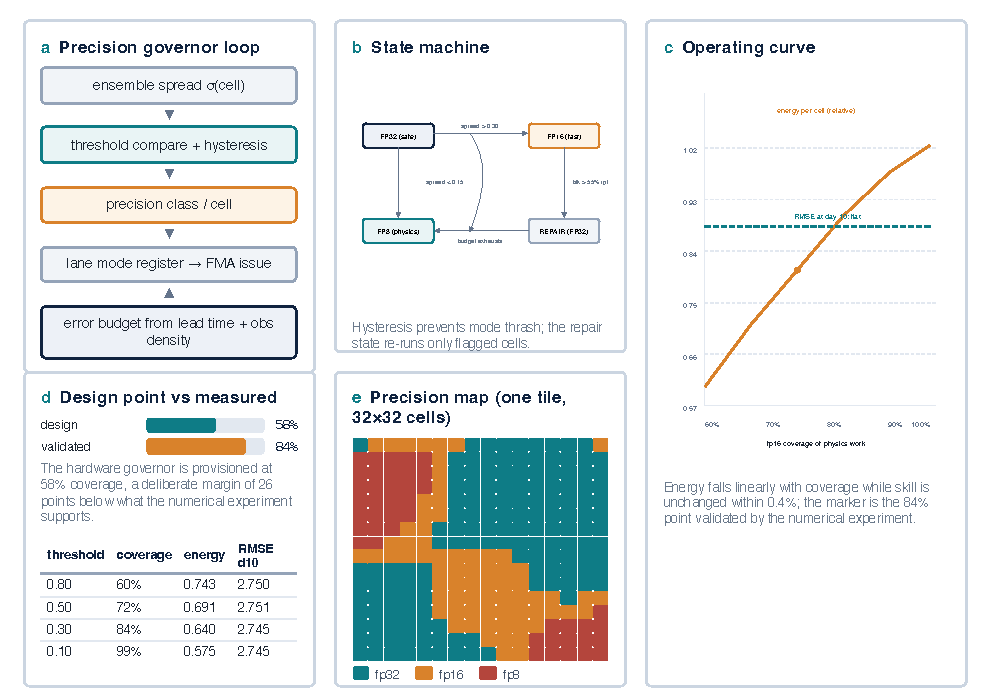
\includegraphics[width=\linewidth]{fig07_precision}
\caption{Precision governor. (a) Control loop from ensemble spread to lane mode. (b) State machine
with hysteresis and a repair state. (c) Operating curve: energy falls linearly with fp16 coverage
while day-10 skill is flat within 0.4\%. (d) Design point (58\%) against the coverage validated by
the numerical experiment (84\%). (e) A tile's precision map; the structure follows the spread
field, not a fixed pattern.}
\label{fig:precision}
\end{figure}

The design point is deliberately conservative. The experiment supports 84\% coverage at no skill
cost; the hardware governor is provisioned for 58\%, a margin of 26 points that covers regimes the
Lorenz--96 surrogate does not represent (fronts, convection, data-sparse oceans). The energy model
uses 58\%, so the projected advantage is not inflated by the best case.

\subsection{Energy accounting}
The energy of a step is the sum of arithmetic, SRAM, L2, L3, HBM, NoC, SFU and static terms:
\begin{equation}
E = \sum_k N_k\,e_k + \sum_{\ell} B_\ell\,e_\ell + P_{\mathrm{static}}\,t .
\end{equation}
Table~\ref{tab:energy} gives the result for W1. HBM is 56\% of the energy; arithmetic is 26\%;
static is 15\%. This is the opposite of the usual accelerator story and it drives the design:
bytes first, reuse second, precision third.

\begin{table}[t]
\centering\small
\caption{Energy breakdown of the reference forecast (7.17 kJ) and the same workload on an H100
(73.0 kJ). The H100 column is derived from its power state model; its HBM share is smaller because
its compute share is much larger.}
\label{tab:energy}
\begin{tabular}{@{}lrr@{}}
\toprule
Component & ACPU-1 & H100 (model)\\
\midrule
Arithmetic & 1.86 kJ (26\%) & 56.9 kJ (78\%)\\
HBM traffic & 4.01 kJ (56\%) & 16.1 kJ (22\%)\\
SRAM / L2 / L3 / NoC & 0.50 kJ (7\%) & ---\\
Static and clock & 1.07 kJ (15\%) & ---\\
Input/output & 0.01 kJ & ---\\
\midrule
Total & 7.17 kJ & 73.0 kJ\\
\bottomrule
\end{tabular}
\end{table}

\subsection{Attribution}
Ablating one feature at a time (Section~\ref{sec:results}) gives the marginal contribution of each
mechanism. Disabling the halo fabric raises energy by 30\% and time by 53\%, because halos then
round-trip through L3. Disabling the precision governor raises energy by 4.3\%. Replacing
ensemble-member lanes with grid-point lanes raises energy by 4.6\% and reduces reuse. Disabling
everything yields 11.05 kJ, 54\% above the full design. The mechanisms are not additive; they
overlap, and the report quotes the full-factorial result rather than a product of factors.
